\documentclass[a3paper,landscape]{article}
\usepackage[margin=1cm]{geometry}
\usepackage[utf8]{inputenc}
\usepackage{tikz}
\usetikzlibrary{calc,positioning,decorations.markings,arrows.meta,backgrounds}
\usepackage{xcolor}
\pagestyle{empty}

% ── Colour palette ──────────────────────────────────────────────
\definecolor{bestblue}{HTML}{1565C0}
\definecolor{okgreen}{HTML}{2E7D32}
\definecolor{failred}{HTML}{C62828}
\definecolor{untriedy}{HTML}{F9A825}
\definecolor{ringgray}{HTML}{BDBDBD}
\definecolor{dirlabel}{HTML}{37474F}
\definecolor{bgcream}{HTML}{FAFAFA}

\begin{document}

% ================================================================
% DIAGRAM 1 — EXPLORATION MAP: WHAT WE TRIED
% ================================================================
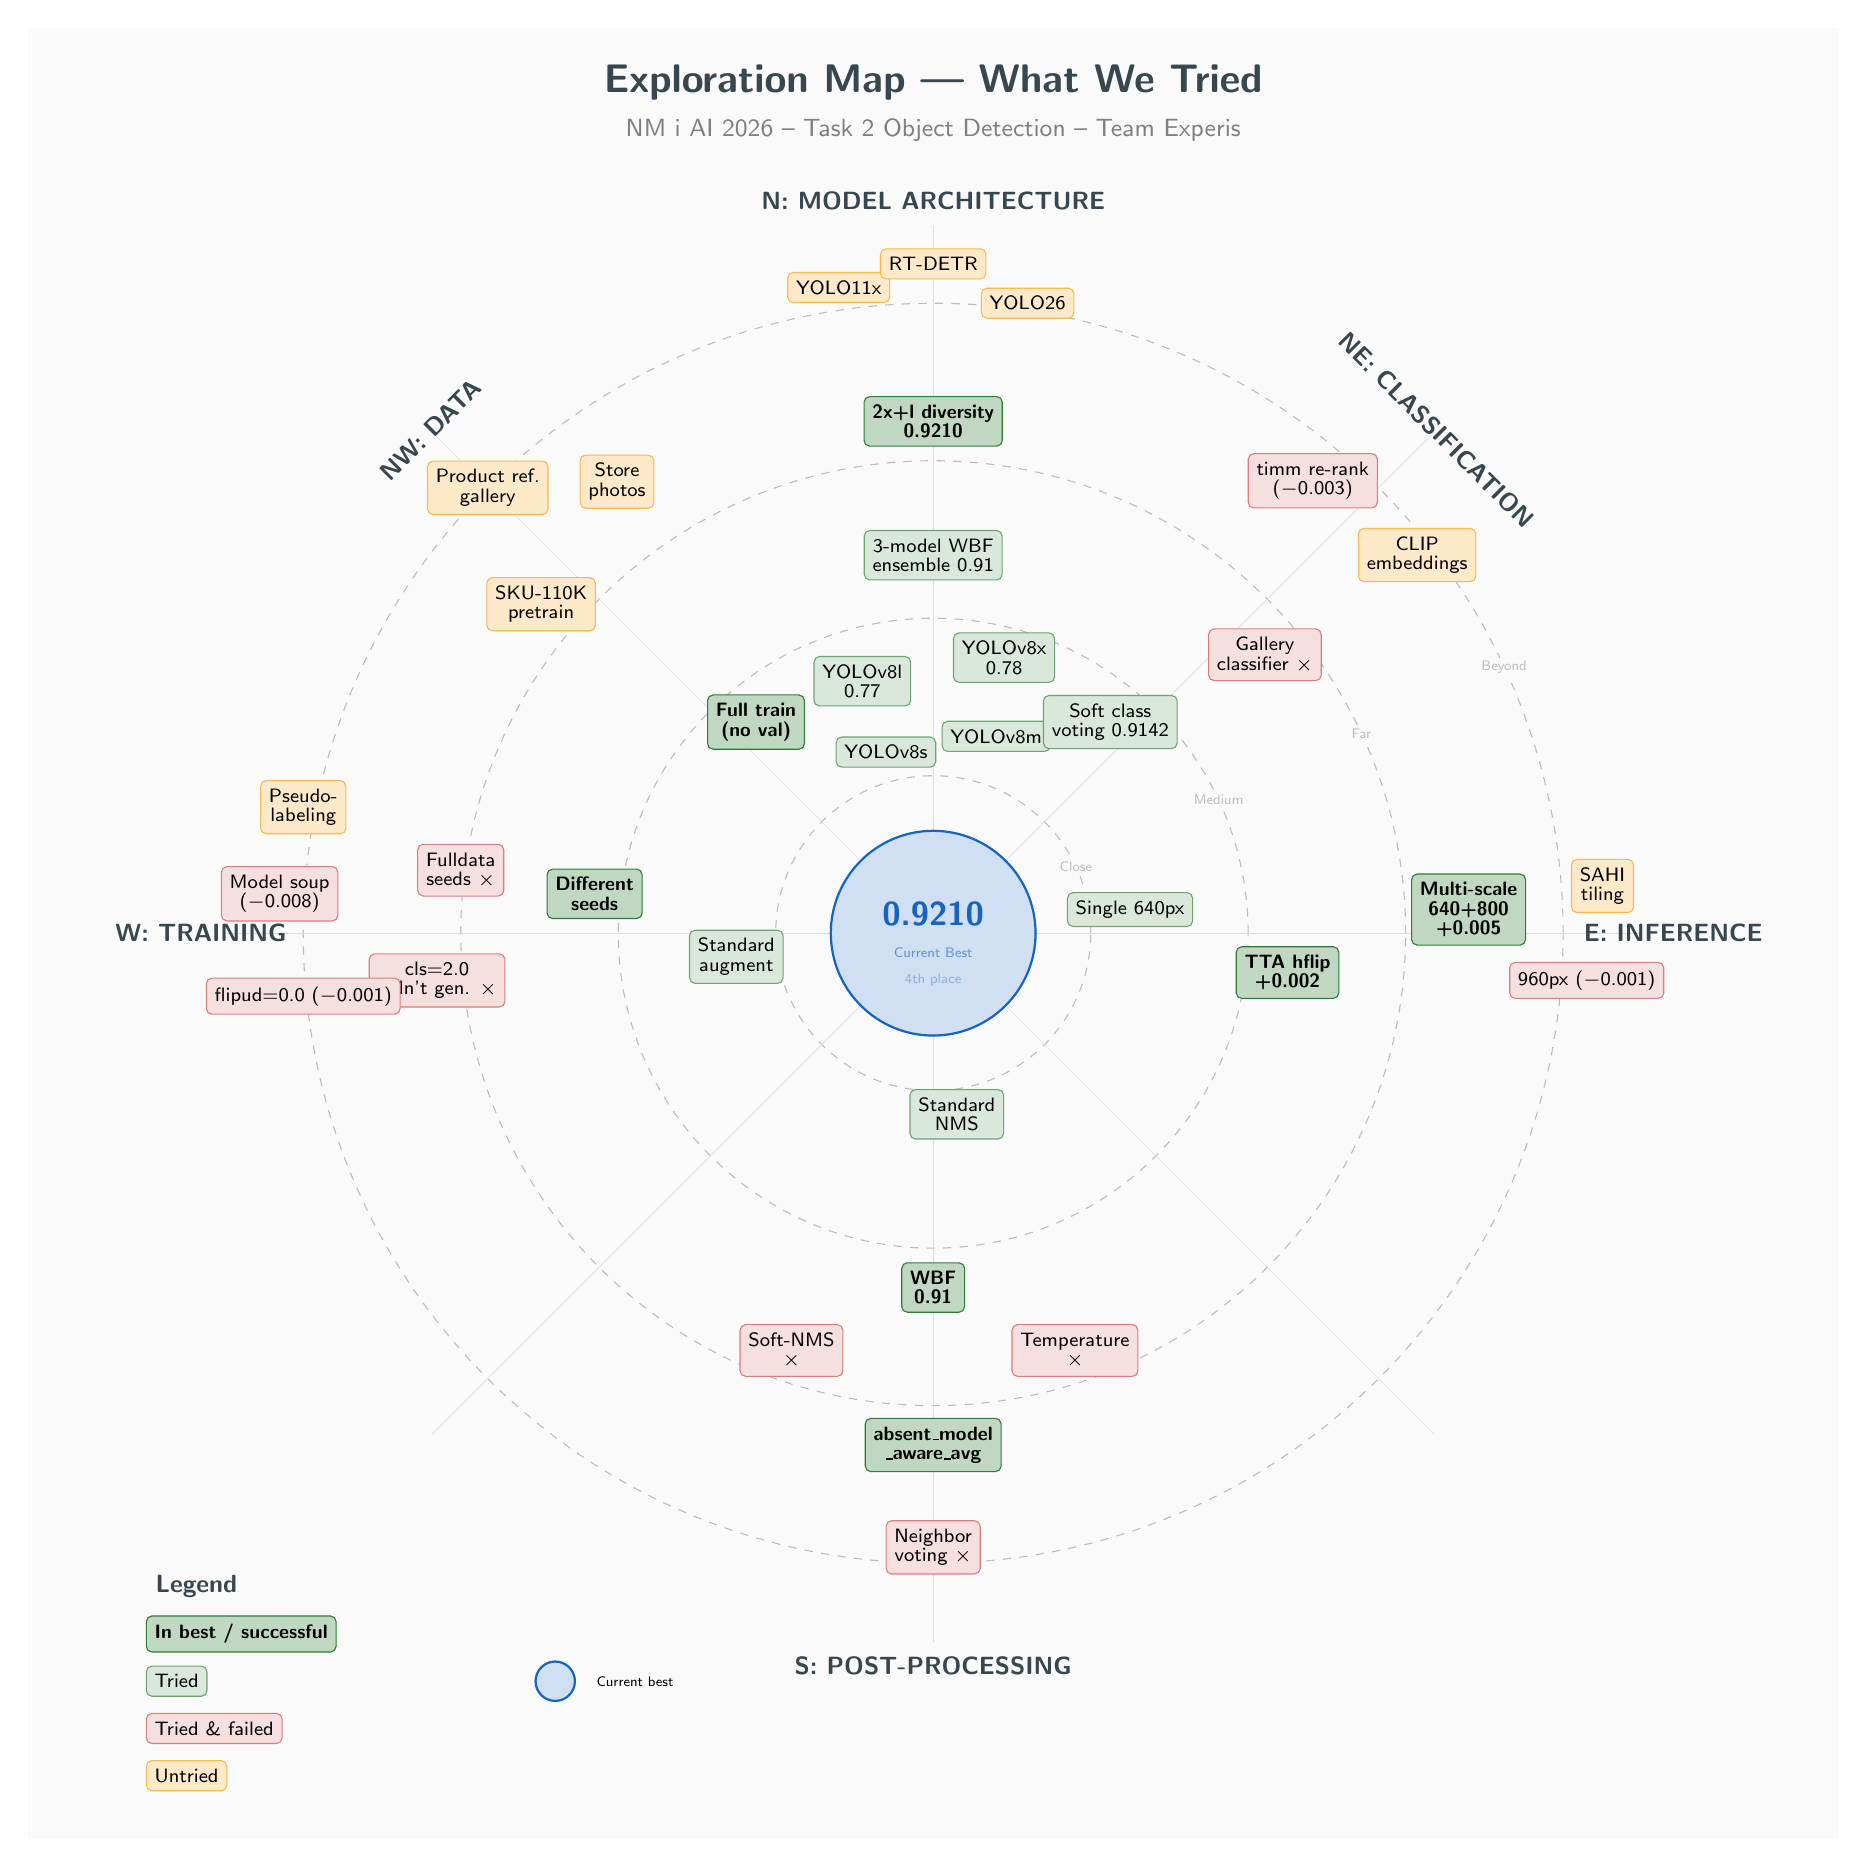
\begin{tikzpicture}[
    remember picture,
    every node/.style={font=\sffamily},
    tried/.style={fill=okgreen!18, draw=okgreen!70, rounded corners=2pt,
                  font=\sffamily\scriptsize, inner sep=3pt, align=center},
    best/.style={fill=okgreen!30, draw=okgreen, rounded corners=2pt,
                 font=\sffamily\scriptsize\bfseries, inner sep=3pt, align=center},
    failed/.style={fill=failred!15, draw=failred!60, rounded corners=2pt,
                   font=\sffamily\scriptsize, inner sep=3pt, align=center},
    untried/.style={fill=untriedy!25, draw=untriedy!80, rounded corners=2pt,
                    font=\sffamily\scriptsize, inner sep=3pt, align=center},
    dirlbl/.style={font=\sffamily\small\bfseries, color=dirlabel},
]

% ── Background ──────────────────────────────────────────────────
\begin{scope}[on background layer]
  \fill[bgcream] (-11.5,-11.5) rectangle (11.5,11.5);
\end{scope}

% ── Title ───────────────────────────────────────────────────────
\node[font=\sffamily\Large\bfseries, color=dirlabel] at (0,10.8)
  {Exploration Map --- What We Tried};
\node[font=\sffamily\small, color=black!50] at (0,10.2)
  {NM i AI 2026 -- Task 2 Object Detection -- Team Experis};

% ── Concentric radar rings ──────────────────────────────────────
\foreach \r/\lbl in {2/Close, 4/Medium, 6/Far, 8/Beyond}{
  \draw[ringgray, thin, dashed] (0,0) circle (\r);
  \node[font=\sffamily\tiny, color=ringgray, fill=bgcream, inner sep=1pt]
    at ({\r*cos(25)},{\r*sin(25)}) {\lbl};
}

% ── Compass axis lines ─────────────────────────────────────────
\foreach \a in {0,45,...,315}{
  \draw[ringgray!50, very thin] (0,0) -- ({9*cos(\a)},{9*sin(\a)});
}

% ── Center node ─────────────────────────────────────────────────
\fill[bestblue!20] (0,0) circle (1.3);
\draw[bestblue, thick] (0,0) circle (1.3);
\node[font=\sffamily\large\bfseries, color=bestblue] at (0,0.25) {0.9210};
\node[font=\sffamily\tiny, color=bestblue!70] at (0,-0.25) {Current Best};
\node[font=\sffamily\tiny, color=bestblue!50] at (0,-0.6) {4th place};

% ════════════════════════════════════════════════════════════════
% NORTH (90°): Model Architecture
% ════════════════════════════════════════════════════════════════
\node[dirlbl] at (0,9.3) {N: MODEL ARCHITECTURE};

\node[tried] at (-0.6, 2.3) {YOLOv8s};
\node[tried] at (0.8, 2.5) {YOLOv8m};
\node[tried] at (-0.9, 3.2) {YOLOv8l\\[-1pt]\scriptsize 0.77};
\node[tried] at (0.9, 3.5) {YOLOv8x\\[-1pt]\scriptsize 0.78};

\node[tried] at (0, 4.8) {3-model WBF\\[-1pt]\scriptsize ensemble 0.91};

\node[best] at (0, 6.5) {2x+l diversity\\[-1pt]\scriptsize \textbf{0.9210} \checkmark};

\node[untried] at (-1.2, 8.2) {YOLO11x};
\node[untried] at (0, 8.5) {RT-DETR};
\node[untried] at (1.2, 8.0) {YOLO26};

% ════════════════════════════════════════════════════════════════
% EAST (0°): Inference Strategy
% ════════════════════════════════════════════════════════════════
\node[dirlbl] at (9.4,0) {E: INFERENCE};

\node[tried] at (2.5, 0.3) {Single 640px};

\node[best] at (4.5, -0.5) {TTA hflip\\[-1pt]\scriptsize +0.002 \checkmark};

\node[best] at (6.8, 0.3) {Multi-scale\\[-1pt]\scriptsize 640+800\\[-1pt]\scriptsize +0.005 \checkmark};

\node[failed] at (8.3, -0.6) {960px ($-$0.001)};
\node[untried] at (8.5, 0.6) {SAHI\\[-1pt]\scriptsize tiling};

% ════════════════════════════════════════════════════════════════
% SOUTH (270°): Post-Processing
% ════════════════════════════════════════════════════════════════
\node[dirlbl] at (0,-9.3) {S: POST-PROCESSING};

\node[tried] at (0.3, -2.3) {Standard\\[-1pt]\scriptsize NMS};

\node[best] at (0, -4.5) {WBF\\[-1pt]\scriptsize 0.91 \checkmark};

\node[best] at (0, -6.5) {absent\_model\\[-1pt]\scriptsize \_aware\_avg \checkmark};

\node[failed] at (-1.8, -5.3) {Soft-NMS\\[-1pt]\scriptsize $\times$};
\node[failed] at (1.8, -5.3) {Temperature\\[-1pt]\scriptsize $\times$};
\node[failed] at (0, -7.8) {Neighbor\\[-1pt]\scriptsize voting $\times$};

% ════════════════════════════════════════════════════════════════
% WEST (180°): Training Strategy
% ════════════════════════════════════════════════════════════════
\node[dirlbl] at (-9.3,0) {W: TRAINING};

\node[tried] at (-2.5, -0.3) {Standard\\[-1pt]\scriptsize augment};

\node[best] at (-4.3, 0.5) {Different\\[-1pt]\scriptsize seeds \checkmark};

\node[failed] at (-6.3, -0.6) {cls=2.0\\[-1pt]\scriptsize didn't gen. $\times$};
\node[failed] at (-6.0, 0.8) {Fulldata\\[-1pt]\scriptsize seeds $\times$};

\node[failed] at (-8.0, -0.8) {flipud=0.0 ($-$0.001)};
\node[failed] at (-8.3, 0.5) {Model soup\\[-1pt]\scriptsize ($-$0.008)};
\node[untried] at (-8.0, 1.6) {Pseudo-\\[-1pt]\scriptsize labeling};

% ════════════════════════════════════════════════════════════════
% NORTHEAST (45°): Classification
% ════════════════════════════════════════════════════════════════
\node[dirlbl, rotate=-45, anchor=south] at ({8.8*cos(45)},{8.8*sin(45)})
  {NE: CLASSIFICATION};

\node[tried] at ({3.5*cos(50)},{3.5*sin(50)}) {Soft class\\[-1pt]\scriptsize voting 0.9142};

\node[failed] at ({5.5*cos(40)},{5.5*sin(40)}) {Gallery\\[-1pt]\scriptsize classifier $\times$};

\node[failed] at ({7.5*cos(50)},{7.5*sin(50)}) {timm re-rank\\[-1pt]\scriptsize ($-$0.003)};
\node[untried] at ({7.8*cos(38)},{7.8*sin(38)}) {CLIP\\[-1pt]\scriptsize embeddings};

% ════════════════════════════════════════════════════════════════
% NORTHWEST (135°): Data
% ════════════════════════════════════════════════════════════════
\node[dirlbl, rotate=45, anchor=south] at ({8.8*cos(135)},{8.8*sin(135)})
  {NW: DATA};

\node[best] at ({3.5*cos(130)},{3.5*sin(130)}) {Full train\\[-1pt]\scriptsize (no val) \checkmark};

\node[untried] at ({6.5*cos(140)},{6.5*sin(140)}) {SKU-110K\\[-1pt]\scriptsize pretrain};
\node[untried] at ({7.0*cos(125)},{7.0*sin(125)}) {Store\\[-1pt]\scriptsize photos};
\node[untried] at ({8.0*cos(135)},{8.0*sin(135)}) {Product ref.\\[-1pt]\scriptsize gallery};

% ── Legend ──────────────────────────────────────────────────────
\begin{scope}[shift={(-10,-9.5)}]
  \node[font=\sffamily\small\bfseries, color=dirlabel, anchor=west] at (0,1.2) {Legend};
  \node[best, anchor=west] at (0, 0.6) {In best / successful};
  \node[tried, anchor=west] at (0, 0) {Tried};
  \node[failed, anchor=west] at (0, -0.6) {Tried \& failed};
  \node[untried, anchor=west] at (0, -1.2) {Untried};
  \draw[bestblue, thick, fill=bestblue!20] (5.2,0) circle (0.25);
  \node[font=\sffamily\tiny, anchor=west] at (5.6,0) {Current best};
\end{scope}

\end{tikzpicture}

\newpage

% ================================================================
% DIAGRAM 2 — FUTURE OPPORTUNITY MAP
% ================================================================
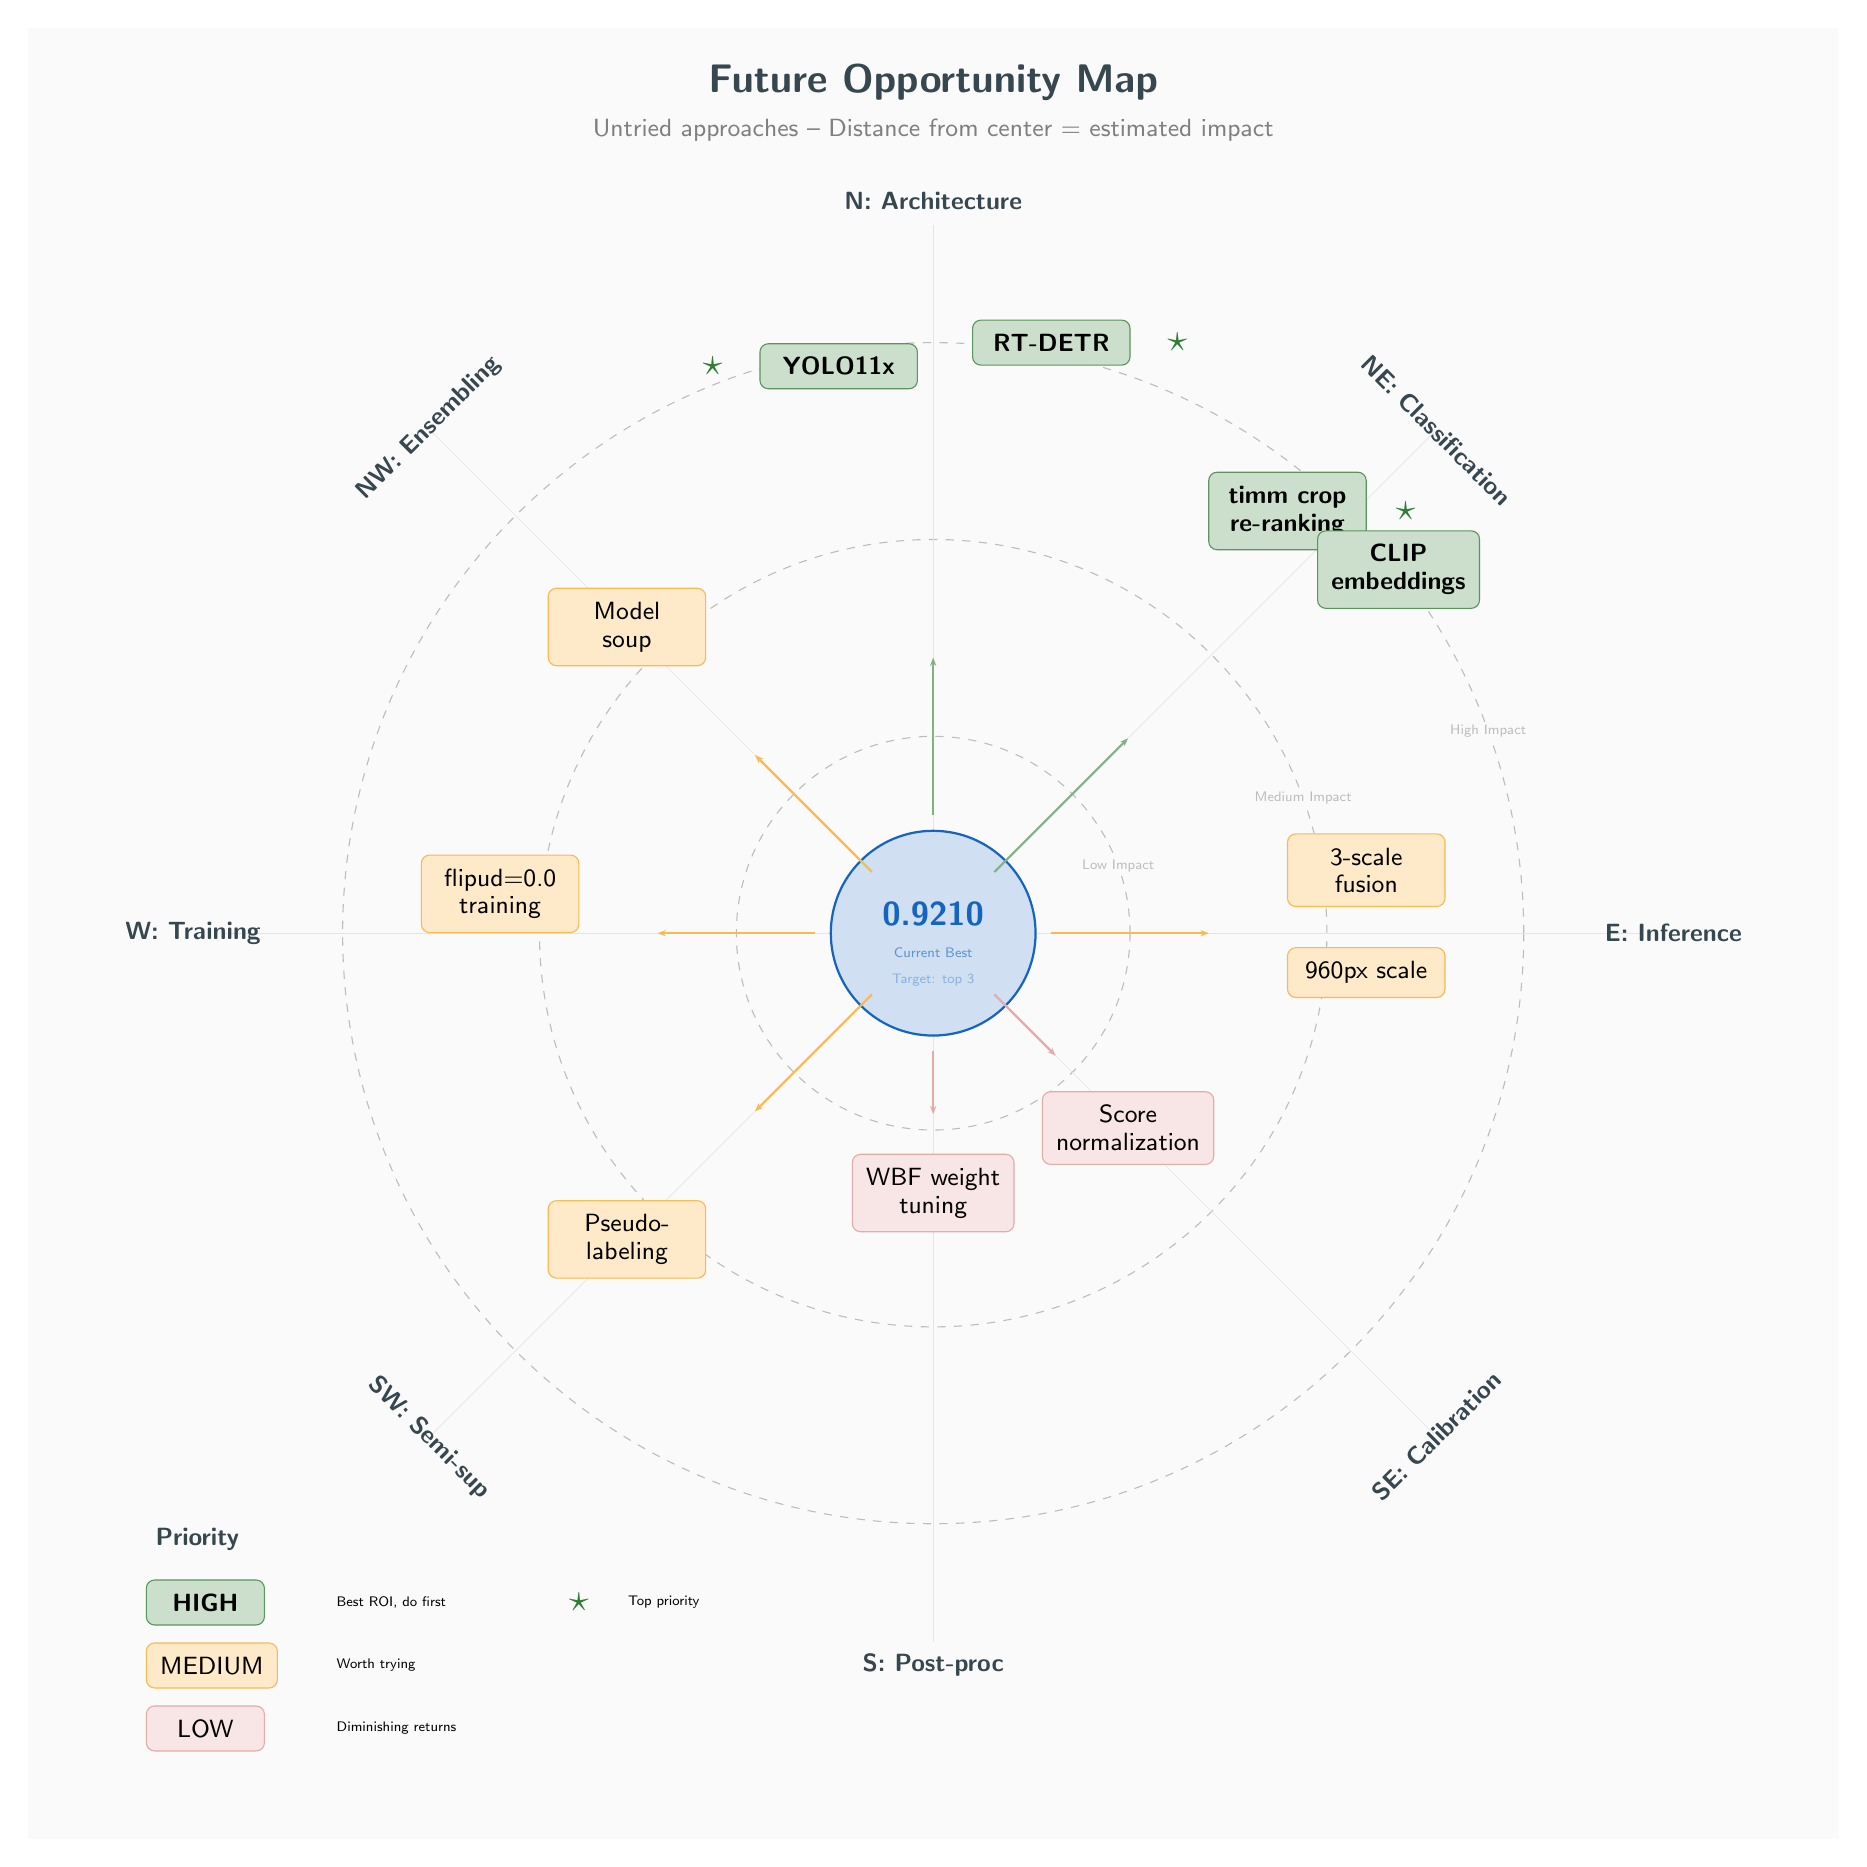
\begin{tikzpicture}[
    remember picture,
    every node/.style={font=\sffamily},
    high/.style={fill=okgreen!25, draw=okgreen!80, rounded corners=3pt,
                 font=\sffamily\small\bfseries, inner sep=5pt, align=center,
                 minimum width=2cm},
    medium/.style={fill=untriedy!25, draw=untriedy!80, rounded corners=3pt,
                   font=\sffamily\small, inner sep=5pt, align=center,
                   minimum width=2cm},
    low/.style={fill=failred!12, draw=failred!40, rounded corners=3pt,
                font=\sffamily\small, inner sep=5pt, align=center,
                minimum width=2cm},
    dirlbl/.style={font=\sffamily\small\bfseries, color=dirlabel},
]

% ── Background ──────────────────────────────────────────────────
\begin{scope}[on background layer]
  \fill[bgcream] (-11.5,-11.5) rectangle (11.5,11.5);
\end{scope}

% ── Title ───────────────────────────────────────────────────────
\node[font=\sffamily\Large\bfseries, color=dirlabel] at (0,10.8)
  {Future Opportunity Map};
\node[font=\sffamily\small, color=black!50] at (0,10.2)
  {Untried approaches -- Distance from center = estimated impact};

% ── Concentric rings with impact labels ─────────────────────────
\foreach \r/\lbl in {2.5/Low Impact, 5/Medium Impact, 7.5/High Impact}{
  \draw[ringgray, thin, dashed] (0,0) circle (\r);
  \node[font=\sffamily\tiny, color=ringgray, fill=bgcream, inner sep=1pt]
    at ({\r*cos(20)},{\r*sin(20)}) {\lbl};
}

% ── Compass axes ────────────────────────────────────────────────
\foreach \a in {0,45,...,315}{
  \draw[ringgray!40, very thin] (0,0) -- ({9*cos(\a)},{9*sin(\a)});
}

% ── Center ──────────────────────────────────────────────────────
\fill[bestblue!20] (0,0) circle (1.3);
\draw[bestblue, thick] (0,0) circle (1.3);
\node[font=\sffamily\large\bfseries, color=bestblue] at (0,0.25) {0.9210};
\node[font=\sffamily\tiny, color=bestblue!70] at (0,-0.25) {Current Best};
\node[font=\sffamily\tiny, color=bestblue!50] at (0,-0.6) {Target: top 3};

% ── Direction labels ────────────────────────────────────────────
\node[dirlbl] at (0, 9.3) {N: Architecture};
\node[dirlbl, rotate=-45, anchor=south] at ({8.8*cos(45)},{8.8*sin(45)}) {NE: Classification};
\node[dirlbl] at (9.4, 0) {E: Inference};
\node[dirlbl, rotate=45, anchor=north] at ({8.8*cos(-45)},{8.8*sin(-45)}) {SE: Calibration};
\node[dirlbl] at (0, -9.3) {S: Post-proc};
\node[dirlbl, rotate=-45, anchor=north] at ({8.8*cos(225)},{8.8*sin(225)}) {SW: Semi-sup};
\node[dirlbl] at (-9.4, 0) {W: Training};
\node[dirlbl, rotate=45, anchor=south] at ({8.8*cos(135)},{8.8*sin(135)}) {NW: Ensembling};

% ── N: Architecture (HIGH) ─────────────────────────────────────
\node[high] at (-1.2, 7.2) {YOLO11x};
\node[high] at (1.5, 7.5) {RT-DETR};

% Draw connecting arrows from center direction
\draw[-{Stealth[length=3pt]}, okgreen!60, thick]
  (0,1.5) -- (0,3.5);

% ── NE: Classification (HIGH) ──────────────────────────────────
\node[high] at ({7*cos(50)},{7*sin(50)}) {timm crop\\[-1pt] re-ranking};
\node[high] at ({7.5*cos(38)},{7.5*sin(38)}) {CLIP\\[-1pt] embeddings};

\draw[-{Stealth[length=3pt]}, okgreen!60, thick]
  ({1.1*cos(45)},{1.1*sin(45)}) -- ({3.5*cos(45)},{3.5*sin(45)});

% ── E: Inference (MEDIUM) ──────────────────────────────────────
\node[medium] at (5.5, -0.5) {960px scale};
\node[medium] at (5.5, 0.8) {3-scale\\[-1pt] fusion};

\draw[-{Stealth[length=3pt]}, untriedy!80, thick]
  (1.5,0) -- (3.5,0);

% ── SE: Calibration (LOW) ──────────────────────────────────────
\node[low] at ({3.5*cos(-45)},{3.5*sin(-45)}) {Score\\[-1pt] normalization};

\draw[-{Stealth[length=3pt]}, failred!40, thick]
  ({1.1*cos(-45)},{1.1*sin(-45)}) -- ({2.2*cos(-45)},{2.2*sin(-45)});

% ── S: Post-processing (LOW) ───────────────────────────────────
\node[low] at (0, -3.3) {WBF weight\\[-1pt] tuning};

\draw[-{Stealth[length=3pt]}, failred!40, thick]
  (0,-1.5) -- (0,-2.3);

% ── SW: Semi-supervised (MEDIUM) ───────────────────────────────
\node[medium] at ({5.5*cos(225)},{5.5*sin(225)}) {Pseudo-\\[-1pt] labeling};

\draw[-{Stealth[length=3pt]}, untriedy!80, thick]
  ({1.1*cos(225)},{1.1*sin(225)}) -- ({3.2*cos(225)},{3.2*sin(225)});

% ── W: Training (MEDIUM) ───────────────────────────────────────
\node[medium] at (-5.5, 0.5) {flipud=0.0\\[-1pt] training};

\draw[-{Stealth[length=3pt]}, untriedy!80, thick]
  (-1.5,0) -- (-3.5,0);

% ── NW: Ensembling (MEDIUM) ────────────────────────────────────
\node[medium] at ({5.5*cos(135)},{5.5*sin(135)}) {Model\\[-1pt] soup};

\draw[-{Stealth[length=3pt]}, untriedy!80, thick]
  ({1.1*cos(135)},{1.1*sin(135)}) -- ({3.2*cos(135)},{3.2*sin(135)});

% ── Priority star annotations ──────────────────────────────────
\node[font=\Large, color=okgreen] at (-2.8, 7.2) {$\star$};
\node[font=\Large, color=okgreen] at (3.1, 7.5) {$\star$};
\node[font=\Large, color=okgreen] at ({7*cos(50)+1.5},{7*sin(50)}) {$\star$};

% ── Legend ──────────────────────────────────────────────────────
\begin{scope}[shift={(-10,-9.5)}]
  \node[font=\sffamily\small\bfseries, color=dirlabel, anchor=west] at (0,1.8) {Priority};
  \node[high, anchor=west, minimum width=1.5cm] at (0, 1.0) {HIGH};
  \node[font=\sffamily\tiny, anchor=west] at (2.3,1.0) {Best ROI, do first};
  \node[medium, anchor=west, minimum width=1.5cm] at (0, 0.2) {MEDIUM};
  \node[font=\sffamily\tiny, anchor=west] at (2.3,0.2) {Worth trying};
  \node[low, anchor=west, minimum width=1.5cm] at (0, -0.6) {LOW};
  \node[font=\sffamily\tiny, anchor=west] at (2.3,-0.6) {Diminishing returns};
  \node[font=\Large, color=okgreen] at (5.5, 1.0) {$\star$};
  \node[font=\sffamily\tiny, anchor=west] at (6.0,1.0) {Top priority};
\end{scope}

\end{tikzpicture}

\end{document}
